\documentclass{article}
\usepackage{cmap}
\usepackage[utf8]{inputenc}
\usepackage[english,ukrainian]{babel}
\usepackage{graphicx}
\usepackage{geometry}
\usepackage{listings}
\usepackage{indentfirst}
\usepackage{subfigure}
\usepackage{caption}
\usepackage{amsmath}
\geometry{
	a4paper,
	left=20mm,
	right=20mm,
	top=20mm,
	bottom=20mm
}
\lstset{
	extendedchars=\true,
	tabsize=4,
	language=python,
	showstringspaces=false,
	showtabs=false,
	frame=lrtb,
	columns=fixed,
	keepspaces,
	breaklines=true
}
\graphicspath{ {pictures} }
\setlength{\parindent}{4em}
\newcommand\subject{Чисельні методи}
\newcommand\lecturer{доцент кафедри ПЗ\\Мельник Н.Б.}
\newcommand\teacher{асистент кафедри ПЗ\\Гарматій Г.Ю.}
\newcommand\mygroup{ПЗ-16}
\newcommand\lab{2}
\newcommand\theme{Розв’язування нелінійних рівнянь методом дотичних та методом послідовних наближень}
\newcommand\purpose{Ознайомлення на практиці з методом дотичних та методом
	послідовних наближень для розв’язування нелінійних рівнянь}

\begin{document}
\begin{large}
	\begin{titlepage}
		\thispagestyle{empty}
		\begin{center}
			\textbf{МІНІСТЕРСТВО ОСВІТИ І НАУКИ УКРАЇНИ\\
				НАЦІОНАЛЬНИЙ УНІВЕРСИТЕТ "ЛЬВІВСЬКА ПОЛІТЕХНІКА"}
		\end{center}
		\begin{flushright}
			Інститут \textbf{КНІТ}\\
			Кафедра \textbf{ПЗ}
		\end{flushright}
		\vspace{200pt}
		\begin{center}
			\textbf{ЗВІТ}\\
			\vspace{10pt}
			До лабораторної роботи № \lab\\
			\textbf{На тему}: “\textit{\theme}”\\
			\textbf{З дисципліни}: “\subject”
		\end{center}
		\vspace{90pt}
		\begin{flushright}
			
			\textbf{Лектор}:\\
			\lecturer\\
			\vspace{28pt}
			\textbf{Виконав}:\\
			
			студент групи \mygroup\\
			Коваленко Д.М.\\
			\vspace{28pt}
			\textbf{Прийняла}:\\
			
			\teacher\\
			
			\vspace{28pt}
			«\rule{1cm}{0.15mm}» \rule{1.5cm}{0.15mm} 2022 р.\\
			$\sum$ = \rule{1cm}{0.15mm}……………\\
			
		\end{flushright}
		\vspace{\fill}
		\begin{center}
			\textbf{Львів — 2022}
		\end{center}
	\end{titlepage}
		
	\begin{description}
		\item[Тема.] \theme.
		\item[Мета.] \purpose.
	\end{description}
	
	\section*{Теоретичні відомості}
	\subsection*{Метод Ньютона (метод дотичних)}
	Запишемо рівняння дотичної до кривої $y = f(x)$ в точці $(x_i;f(x_i))$, де $f(x)$ є
	неперервною монотонною нелінійною функцією, яка на кінцях відрізку $[a,b]$ приймає значення різних знаків, причому її похідні $f'(x)$ та $f''(x)$ є неперервними та монотонними.
	
	\begin{equation}
		y - f(x_i) = f'(x_i)(x-x_i)\nonumber
	\end{equation}
	
	\begin{figure}[h]
		\centering
		\subfigure[]{\includegraphics[width=0.38\textwidth]{1}} 
		\subfigure[]{\includegraphics[width=0.38\textwidth]{2}} 
		\subfigure[]{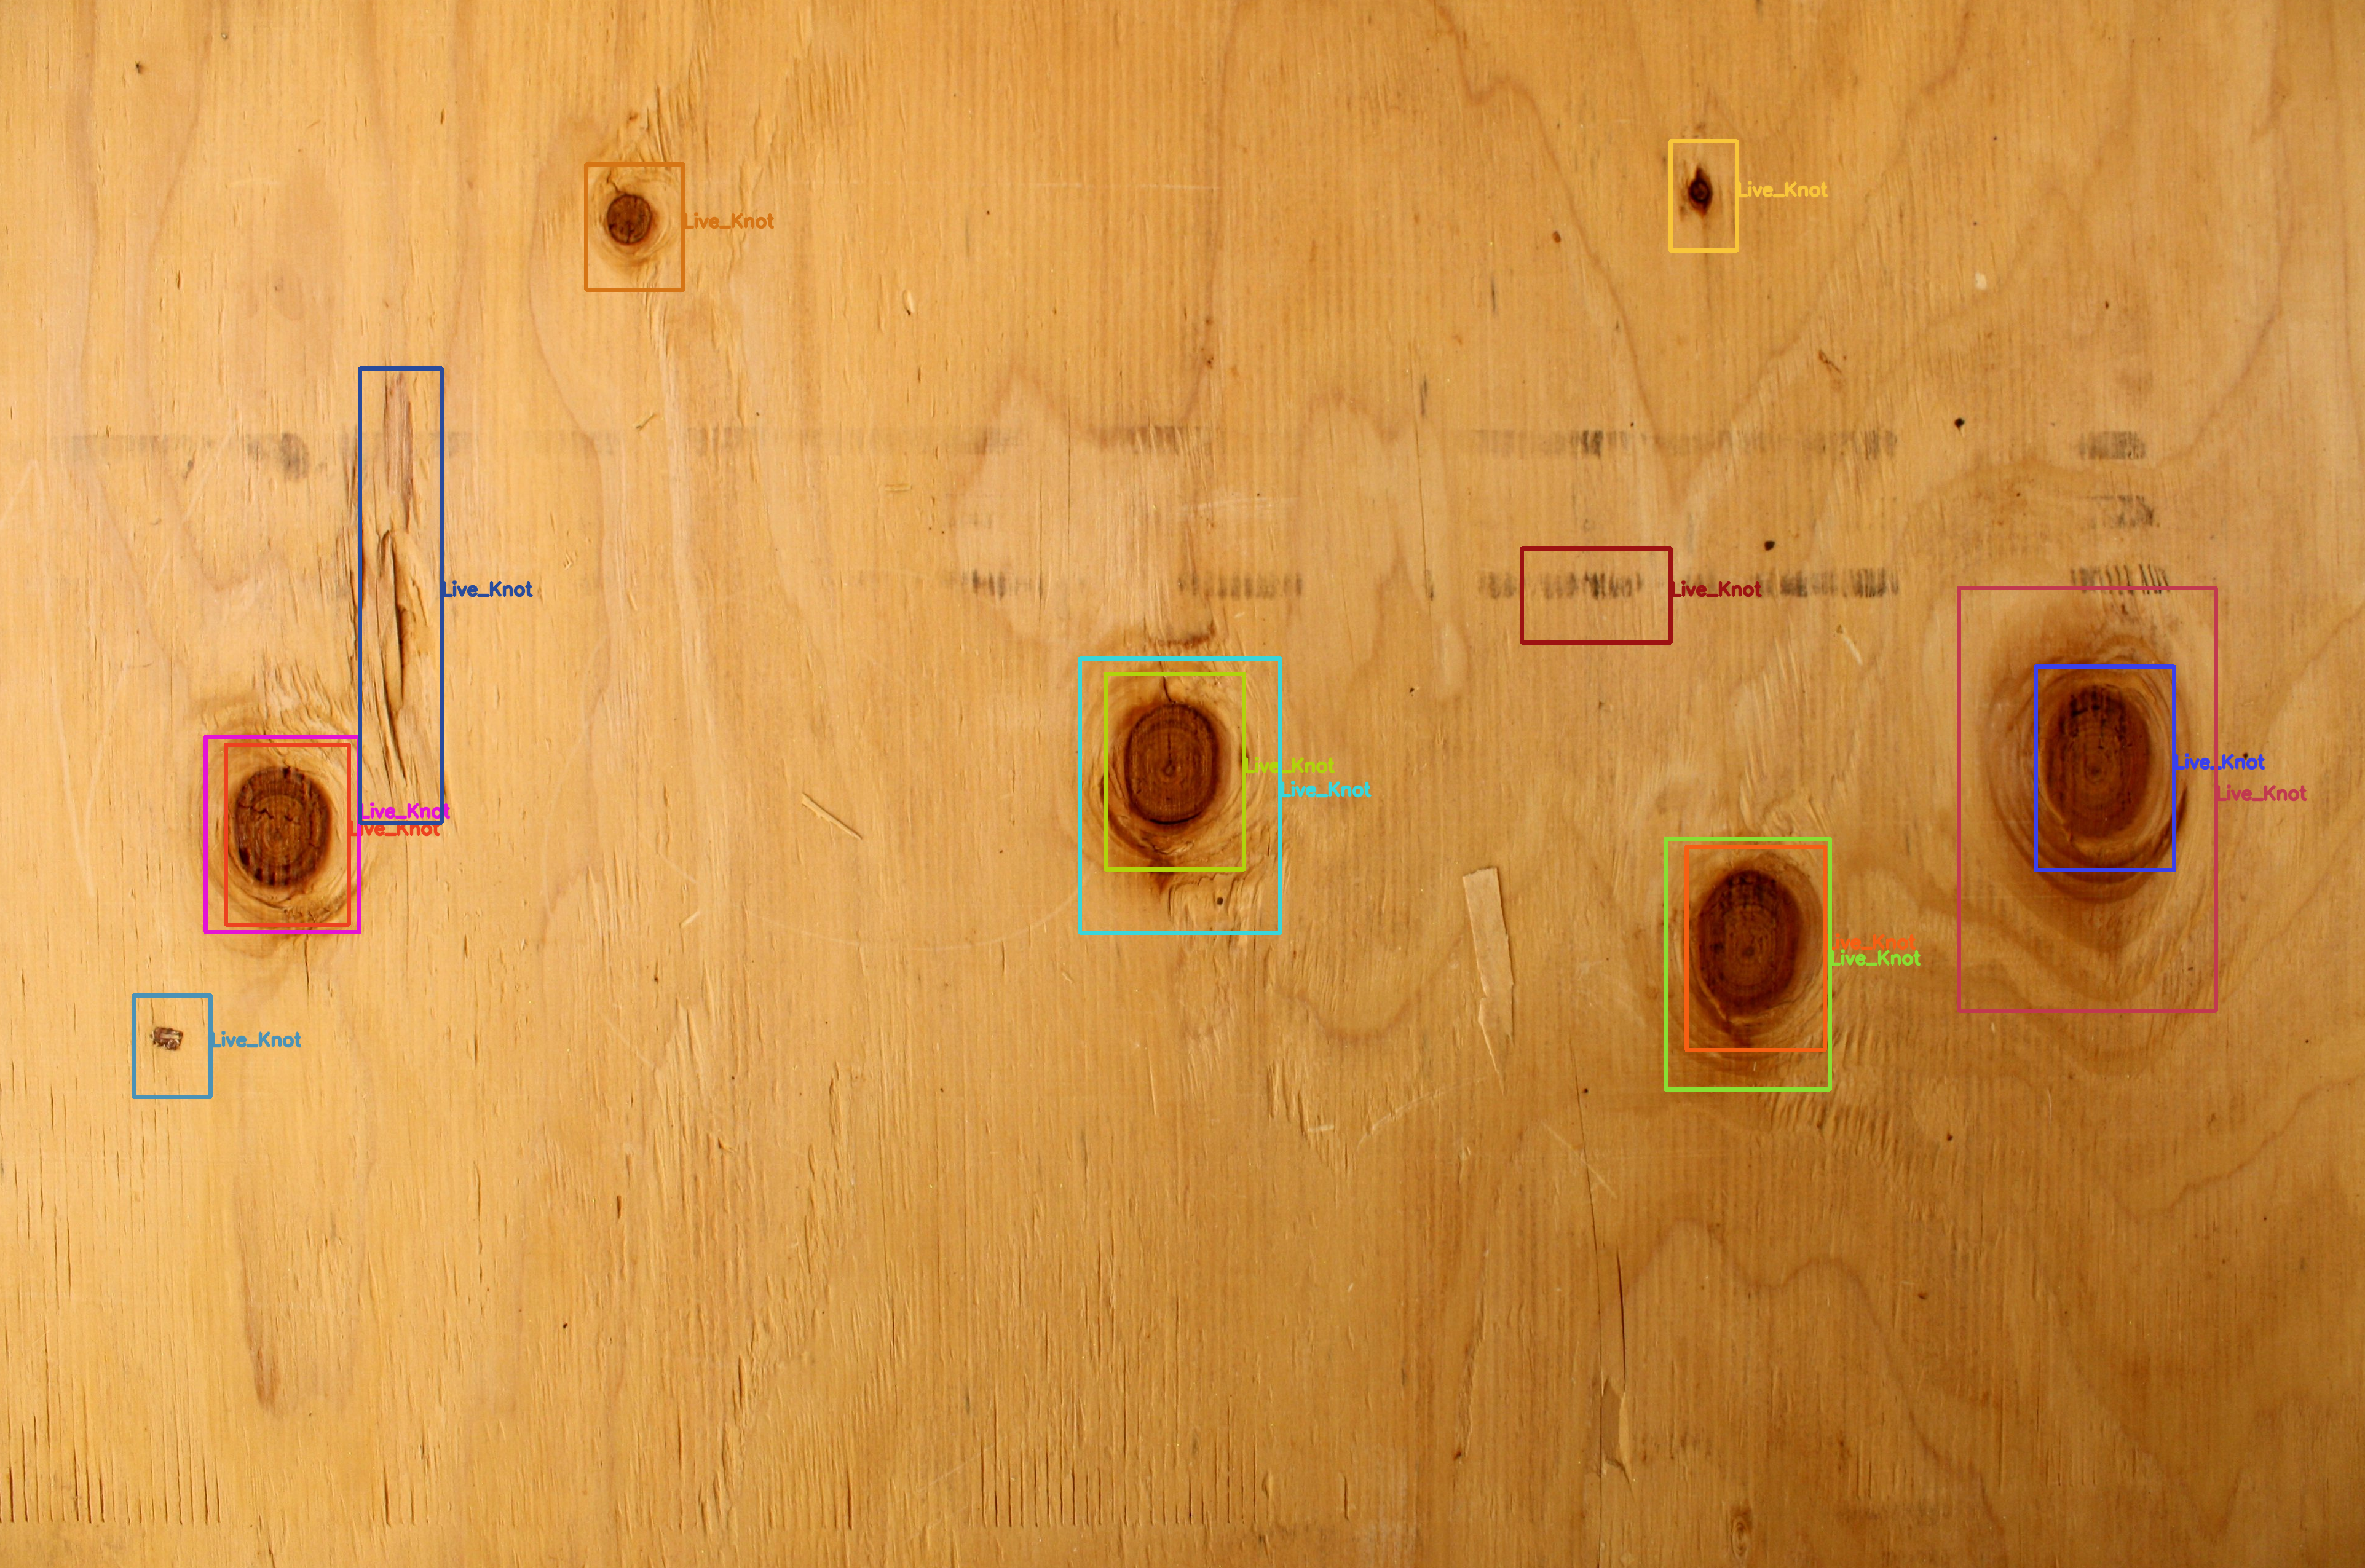
\includegraphics[width=0.38\textwidth]{3}}
		\subfigure[]{\includegraphics[width=0.38\textwidth]{4}}
		\captionsetup{justification=centering}
		\caption{Геометричний зміст методу Ньютона:\\
		а) графік функції $y = f(x)$ є вгнутим ($f'(x)>0;f''(x)>0$);\\
		б)графік функції $y = f(x)$ є опуклим ($f'(x)<0;f''(x)<0$);\\
		в)графік функції $y = f(x)$ є опуклим ($f'(x)>0;f''(x)<0$);\\
		г)графік функції $y = f(x)$ є вгнутим ($f'(x)<0;f''(x)>0$).}
	\end{figure}
	
	Геометричний зміст (рис. 1) методу Ньютона полягає в тому, що дугу кривої $y = f(x)$ на відрізку $[a,b]$ замінюють дотичною до цієї кривої, а наближене значення кореня визначають як абсцису точки перетину дотичної з віссю $Ox$, проведеної через один із кінців відрізка.

	Тоді ітераційні формули запишемо у вигляді
	\begin{equation}
		x_{i+1}=x_i-\frac{f(x_i)}{f'(x_i)}, \hspace{18pt}i=1,2,3...\nonumber
	\end{equation}
	
	Для вибору початкового наближення кореня рівняння $f(x) = 0$ необхідно керуватися таким правилом: за початкову точку слід вибирати той кінець відрізка $[a,b]$ , в якому знак функції $y= f(x)$ співпадає зі знаком її другої похідної $y=f''(x)$.
	
	\subsection*{Метод простої ітерації (метод послідовних наближень)}
	
	Запишемо у рівняння $f(x)=0$ канонічній формі
	\begin{equation}
		x=\phi(x)\nonumber
	\end{equation} 
	
	Довільним способом визначимо найближче значення $x_0$ кореня рівняння і підставимо його у праву частину співвідношення. У результаті одержимо
	\begin{eqnarray}
		x_1=\phi(x_0)\nonumber
	\end{eqnarray}

	Підставимо у праву частину рівняння замість $x_0$ значення $x_1$, тоді $x_2$. Повторюючи цей процес, отримаємо ітераційні формули
	\begin{equation}
		x_i = \phi(x_{i-1}), \hspace{18pt} i=1,2,3...\nonumber
	\end{equation}
	
	Кожний дійсний корінь $x_*$ рівняння є абсцисою точки перетину кривої $y=\phi(x)$ з прямою $y=x$. Доведено що ітераційний процес, визначений формулами, збігається до єдиного кореня
	рівняння $f(x)=0$, якщо на відрізку $[a,b]$, який містить цей корінь, виконано умову:
	\begin{equation}
		|\phi'(x)| \le q = \underset{x\in[a,b]}{max} |\phi'(x)|<1\nonumber
	\end{equation}
	
	\begin{figure}[h]
		\centering
		\includegraphics[width=0.4\textwidth]{5}
		\captionsetup{justification=centering}
		\caption{Геометричний зміст методу ітерацій}
	\end{figure}
	
	\section*{Лабораторне завдання}
	\begin{enumerate}
		\item Ознайомитись з теоретичними відомостями.
		\item Скласти програму розв’язування нелінійного рівняння $x^3-6x^2-7=0$ методом дотичних та методом простої ітерації.
	\end{enumerate}
	
	\section*{Хід роботи}
	\subsection*{Графічний метод}
	\begin{figure}[h!]
		\centering
		\includegraphics[scale=0.5]{8}
		\hfill
		\includegraphics[scale=0.5]{9}
		\caption{Графік функції $y=x^3-6x^2-7$}
	\end{figure}
	За графіком функції (рис. 3) можна зробити висновок, що корінь рівняння належить проміжку $[6,7]$.
	
	\subsection*{Аналітичний метод}
	Для аналітичного розв’язку визначимо монотонність функції f(x), для цього розв’яжемо рівняння $f'(x) = 0$ та знайдемо інтервали монотонності.
	
	$3x^2-12x=0$
	
	Інтервалами монотонності є $(-\infty; 0)$, $(0; 4)$, $(4; +\infty)$. Виберемо лише ті інтервали, де функція змінює знак $f(x) = f(x^3-6x^2-7) = +\infty$, $f(x) = f(x^3-6x^2-7) = -\infty$
	
	$f(4) < 0$, $f(+\infty) > 0$, Отже, $(4; +\infty)$ єдиний відрізок, де є корінь, бо на всіх інших знак не змінюється і функція є монотонною. Це значить, що корінь є і він лежить в цьому інтервалі. Знайдемо відрізок, де є корінь рівняння, для цього перевіримо знак функції у цілочисельних точках інтервалу.
	
	$f(6) = -7 < 0$ та $f(7) = 42 > 0$, отже корінь належить відрізку $[6; 7]$.
	
	\subsection*{Метод дотичних}	
	\noindent\textit{\textbf{Код програми} (файл lab\_21.py):}
	\begin{lstlisting}
class TangentMethod:
	def __init__(self, a, b, eps, f, first_der, second_der):
		self.a = a # Ліва межа
		self.b = b # Права межа
		self.x = 1 # Шукане значення
		self.i = 0 # Кількість ітерацій
		self.eps = eps # Точність
		self.f = f # Функція
		self.first_der = first_der # Перша похідна функції
		self.second_der = second_der # Друга похідна функції
		if a >= b:
			return print("Помилка, 'a' більше або рівне 'b'")
		elif eps > b - a:
			return print("Помилка, 'eps' більше ніж інтервал між 'a' та 'b'")
		elif self.calc_f(f, a) * self.calc_f(self.second_der, a)>0:
			x = a
		else:
			x = b
	
	def calculate(self):
		print(f"x: {self.x} f(x): {self.calc_f(self.f, self.x)} f'(x): {self.calc_f(self.first_der, self.x)}")
		if abs(self.calc_f(self.f, self.x)) < self.eps:
			return f"Відповідь: {self.x} \n Кількість ітерацій: {self.i}"
		else:
			self.i += 1
			self.x -= self.calc_f(self.f, self.x) / self.calc_f(self.first_der, self.x)
			return self.calculate()
	
	def calc_f(self, f, x):
		return eval(f.replace("x", str(x)))
a = float(input("Ліва межа: "))
b = float(input("Права межа: "))
eps = float(input("Точність: "))
f = input("Функція: ") or "x*x*x - 6*x*x - 7"
first_der = input("Перша похідна функції: ") or "3*x*x - 12*x"
second_der = input("Друга похідна функції: ") or "6*x - 12"
print(TangentMethod(a,b,eps, f, first_der, second_der).calculate())\end{lstlisting}
	
	\begin{figure}[h!]
		\centering
		\includegraphics[scale=0.65]{6}
		\caption{Робота програми}
	\end{figure}
	
	\subsection*{Метод простої ітерації}
	Для методу простої ітерації виконаємо деякі перетворення рівняння.
	\begin{gather}
		x^3-6x^2-7=0;\nonumber\\
		x^3=6x^2+7;\nonumber\\
		x=(6x^2+7)^{1/3};\nonumber\\
		\phi(x)=(6x^2+7)^{1/3};\nonumber\\
		\phi'(x) = \frac{4x}{(6x^2+7)^{2/3}}.\nonumber
	\end{gather}
	
	$|\phi'(x)| = |\frac{4x}{(6x^2+7)^{2/3}}| \le 0.65$ для всіх $x\in[6,7]$. Тому ітераційний процес є збіжним.
	
	\noindent\textit{\textbf{Код програми} (файл lab\_22.py):}
	\begin{lstlisting}
class IterationMethod:
	def __init__(self, a, b, eps, f, phi):
		self.a = a # Ліва межа
		self.b = b # Права межа
		self.x = 6.5 # Шукане значеня
		self.i = 0 # Кількість ітерацій
		self.eps = eps # Точність
		self.f = f # Функція
		self.phi = phi # Канонічні форма функції
		
		if a >= b:
			print("Помилка, 'a' більше або рівне 'b'")
			exit(1)
		elif eps > b - a:
			print("Помилка, 'eps' більше ніж інтервал між 'a' та 'b'")
			exit(1)
	
	def calculate(self):
		print(f"x: {self.x} f(x): {self.calc_f(self.f, self.x)}")
		if abs(self.calc_f(self.f, self.x)) < self.eps:
			return f"Відповідь: {self.x} \n Кількість ітерацій: {self.i}"
		else:
			self.i += 1
			self.x = self.calc_f(self.phi, self.x)
			return self.calculate()
	
	def calc_f(self, f, x):
		return eval(f.replace("x", str(x)))

a = float(input("Ліва межа: "))
b = float(input("Права межа: "))
eps = float(input("Точність: "))
f = input("Функція: ") or "x*x*x - 6*x*x - 7"
phi = input("Функція у канонічній формі: ") or "(6*x*x + 7)**(1/3)"

print(IterationMethod(a, b, eps, f, phi).calculate())
\end{lstlisting}
	
	\begin{figure}[h!]
		\centering
		\includegraphics[scale=0.7]{7}
		\caption{Робота програми}
	\end{figure}
	
	\section*{Висновок}
	На лабораторній роботі я засвоїв практичні навички використання методу дотичних та методу послідовних наближень та розробив функції для розв’язку нелінійного рівняння $x^3-6x^2-7$ з точністю $0.001$ за допомогою цих методів. Корінь рівняння 6.183.
	
\end{large}
\end{document}
